\documentclass[b5paper,fleqn,9pt,uplatex]{jsbook}
    %========================
    % パッケージの読み込み
    %========================
      %===============================================================================
% パッケージの読み込み
%===============================================================================
%% ------------------------------------------
%% * Now Setting
%% ------------------------------------------
%\usepackage[setpagesize=false,dvipdfmx,%
%bookmarks=true,bookmarksnumbered=true,%
%bookmarksopen=false,%
%colorlinks=false,%
%pdftitle={タイトル},%
%pdfauthor={作成者},%
%pdfsubject={サブタイトル},%
%pdfkeywords={キーワード},%
%pdfborder={0 0 0},%
%linkcolor=blue,anchorcolor=blue,urlcolor=blue,
%]{hyperref}
%\RequirePackage[12tabu, orthodox]{nag}
%\usepackage{atbegshi}
%\AtBeginShipoutFirst{\special{pdf:tounicode 90ms-RKSJ-UCS2}}
%\usepackage{refcheck}              % ref auto check
\usepackage[dvipdfmx]{graphicx}
%\usepackage{mediabb}               %  pdfの図を挿入時の,大きさの設定を自動化する
%\usepackage{gradientframe}          %  図に影をつける
\usepackage[dvips]{color}           %  dvipsにて,色付文字を有効化する

\usepackage{bm}                     %  数式太字

%\usepackage{lmodern}
\usepackage{fancyhdr}

\usepackage{bbding}
\usepackage{textcomp}
\usepackage{okumacro}
\usepackage{fancybox}               %  囲みの種類の追加
%\usepackage{calrsfs}               %  文字の種類の追加 1
%\usepackage{rsfso}                 %  文字の種類の追加 2
\usepackage{ascmac}                 %  数式環境の拡張
\usepackage{amsfonts}               %  数式の拡張1
\usepackage{amsthm}                 %  数式の拡張2
\usepackage{amsmath,amssymb}        %  数式の拡張3
\usepackage{mathtools}                                %  数式の拡張4
\usepackage[sans]{dsfont}
\usepackage[T1]{fontenc}
\usepackage{pifont}
%  \mathtoolsset{showonlyrefs=true}  %    参照していない式の番号は付加しない
\usepackage{enumitem}
\usepackage[all, warning]{onlyamsmath}
%\usepackage{esvect}                %  その他のベクトル表現
\usepackage{url}                    %  \url のために必要
\usepackage{makeidx}                %  索引のために
%\usepackage{mediabb}               %  PDFファイル読み込みのために
%\usepackage[dvipdfmx]{hyperref}    %  文字化け
%\usepackage[hypertex]{hyperref}    %  動作がおかしい
\usepackage[cc]{titlepic}           %  表紙に図を挿入可能にする
%\usepackage{harmony}               %  音符が表示できるはずだが,フォントが見つからない
%\usepackage{hangcaption}           %  長いキャプションの折り返し
%\usepackage[times]{quotchap}        %  章のみだし体裁の変更
%\usepackage{pdfdraftcopy}          %  透かしを入れる
%  \draftstring{作成中}             %    -> 透かしの文字列 を設定
%\usepackage[brackets]{fnindent}    %  脚注の体裁を変更
\usepackage[version=4]{mhchem}
\usepackage{setspace}               % 行間調整してみる(\setstretch{1.5}, \begin{spacing}{0.8}-\end{spacing})
%\usepackage{breqn}                  % \begin{dmath}
\usepackage{wasysym}
\usepackage{layout}
\usepackage{braket}                 %  ディラックのブラケット
\usepackage{physics}                % 物理でよく使う数式ショートカット

\usepackage{pxrubrica}              % ルビ
\usepackage{plext}
\usepackage[T1]{fontenc}
\usepackage[utf8]{inputenc}

%\usepackage{kpfonts}
%\usepackage{txfonts}               %  Times フォントの使用
%\usepackage{newtxtext,newtxmath}   %  NewTimes フォントの使用
%\usepackage{fourier}               %  アルファベットフォント変更 1
%\usepackage{fouriernc}             %  アルファベットフォント変更 2
%\usepackage{kurier}                %  アルファベットフォント変更 3
%\usepackage{lmodern}               % Latine Modern
\usepackage{pxfonts}                %
% --- End Of Setting ---


%%%%%%%%%%%%%%%%%%%%%%%%%%%%%%%%%%%%%%%%%%%%%%%%%%%%%%%%%%%%%%%%%%%%%%%%%%%%%%%%
%%%%%%%%% Back Up Code %%%%%%%%%%%%%%%%%%%%%%%%%%%%%%%%%%%%%%%%%%%%%%%%%%%%%%%%%
%%%%%%%%%%%%%%%%%%%%%%%%%%%%%%%%%%%%%%%%%%%%%%%%%%%%%%%%%%%%%%%%%%%%%%%%%%%%%%%%
%% ------------------------------------------
%% * Old Setting (hyperref)
%% ------------------------------------------
%\usepackage[dvipdfmx,%
%colorlinks=true,%
%urlcolor=black,%
%linkcolor=black,%
%citecolor=black,%
%linktocpage=true,%
%bookmarkstype=toc,%
%bookmarksdepth=4,%
%bookmarksnumbered=true,%
%bookmarksopen=true,%
%bookmarks=true]{hyperref}
%%\AtBeginDvi{\special{pdf:tounicode EUC-UCS2}}%EUC
%\AtBeginDvi{\special{pdf:tounicode 90ms-RKSJ-UCS2}}%SJIS


    %========================
    % 表紙
    %========================
      %========================
% 表紙
%========================
    \title{
        \Huge{古典力学ノート}
    }

    \author{
        菅谷\;\;\;千慧
    }

    \西暦
    \date{
        \today \quad 更新\\
        {\small (2010年 8月 より作製開始)}
    }
    % 表紙に画像を貼る
    \titlepic{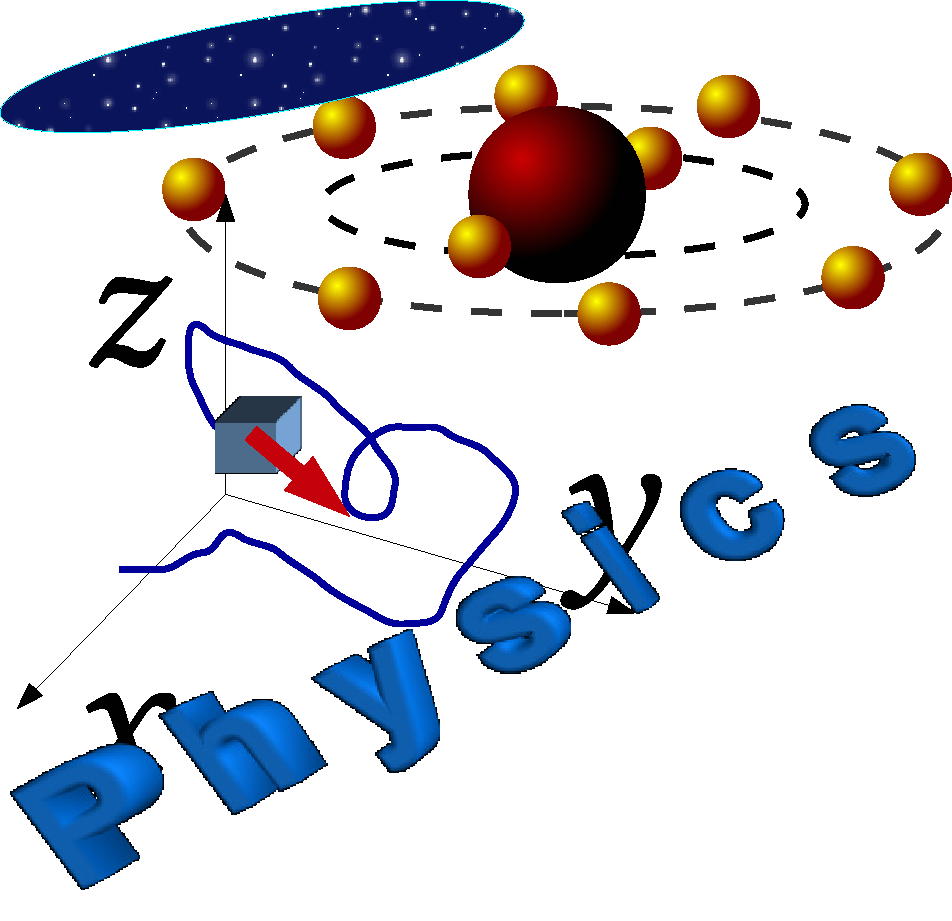
\includegraphics[keepaspectratio, width=6cm,height=3cm,clip]{hyoushi.pdf}}
    \par


    %========================
    % 索引作成の宣言
    %========================
      \makeindex

    %========================
    % 再定義(renewcommand)
    %========================
      %******************************************************************************
%  Newcommand
%******************************************************************************
%================================================
% * 章・節などの表示変更
%================================================
\renewcommand{\thesection}{\thechapter.\arabic{section}}
\renewcommand{\thesubsection}{\thesection.\arabic{subsection}}
\renewcommand{\tablename}{表\;}
\renewcommand{\figurename}{図\;}

\renewcommand{\bibname}{参考図書・教科書等}

%\renewcommand{\prechaptername}{第}
%\renewcommand{\postchaptername}{章}

\renewcommand{\labelenumi}{(\arabic{enumi})\;}
\renewcommand{\labelenumii}{(\alph{enumii})\;}
\renewcommand{\labelenumiii}{(\roman{enumiii})\;}
 %% - 一般の脚注のスタイル変更
%\renewcommand\thefootnote{$\mbox{}^{\clubsuit}$\kern1pt\arabic{footnote})\,} % パターン1: 三つ葉
\renewcommand\thefootnote{$\mbox{}^{\blacktriangleright}$\kern1pt\arabic{footnote})\,} % パターン2: 黒三角形
\renewcommand{\footnoterule}{%
  \vspace{1pt}                      % 線から上の幅
  \noindent\rule{0.25\textwidth}{0.5pt}   % 線の長さ,太さ
  \vspace{2pt}                     % 線から下の幅
}

\renewcommand{\textreferencemark}{\textreferencemark\,\,}
\newcommand{\komemark}{\textreferencemark}
 %% - 行間の調整
%\renewcommand{\baselinestretch}{1.05}%普通のx倍の行間間隔

%================================================
% * 演算子などの省略記述用
%================================================
% * ベクトル解析用の演算子
\newcommand{\drot}{\mathrm{rot}\,}
\newcommand{\ddiv}{\mathrm{div}\,}
\newcommand{\dgrad}{\mathrm{grad}\,}
% * ゼロベクトル
\newcommand{\bzero}{\textbf{0}}
% * 面積分
\newcommand{\sint}{\int\mspace{-11mu}\int}
% * 体積積分
\newcommand{\vint}{\int\mspace{-11mu}\int\mspace{-11mu}\int}
\newcommand{\OmegaS}{\Omega_{S}}
% * 微分記号(立った"d")
\newcommand{\df}{\,\mathrm{d}}
% * 偏微分記号
\newcommand{\rd}{\partial}
% * ダランべルシアン
\newcommand{\Dal}{\Box\,}
% * ラプラシアン
\newcommand{\Lap}{\triangle}
% * 自然対数の底
\newcommand{\e}{\mathrm{e}}
%\newcommand{\exp}{\mathrm{exp}}
% * 量子論的ハミルトニアン記号:$\qH$
\newcommand{\qH}{\mathcal{H}\,}
% * ラグランジアン密度
\newcommand{\qL}{\mathcal{L}\,}
% * 量子論的運動量演算子:$\dpx , \dpy , \dpz$
\newcommand{\dpx}{-i\hbar \frac{\partial}{\partial x}\,}
\newcommand{\dpy}{-i\hbar \frac{\partial}{\partial y}\,}
\newcommand{\dpz}{-i\hbar \frac{\partial}{\partial y}\,}
% * 量子論的エネルギー演算子:$\dE$
\newcommand{\dE}{i\hbar \frac{\partial}{\partial t}\,}
% * 量子論的ハミルトニアン演算子:$\dH$
\newcommand{\dH}{-i\hbar \nabla \,}
% * その他
\newcommand{\Shrps}{$\sharp\;$} % シャープ記号#
\newcommand{\Fig}{Fig\,\,} % 参照図を明示するときに使用する:ex.) 図\ref{xxx}
\newcommand{\Table}{図\,\,}
\newcommand{\circC}{${}^{\circ}$C}

%================================================
% * 標準的な画像のサイズ
%================================================
% 4:3 Default Size
\newcommand{\includegraphicsdefault}[1]{\includegraphics[keepaspectratio, width=4.00cm, height=3.00cm, clip]{#1}}
% 4:3 Middle Size
\newcommand{\includegraphicsmiddle}[1]{\includegraphics[keepaspectratio, width=6.00cm, height=4.5cm, clip]{#1}}
% 4:3 Large Size
\newcommand{\includegraphicslarge}[1]{\includegraphics[keepaspectratio, width=7.2cm, height=4.98cm, clip]{#1}}
% 2:1 Default Size
\newcommand{\includegraphicshalfmid}[1]{\includegraphics[keepaspectratio, width=6cm, height=3cm, clip]{#1}}
% 1:1 Squeare Default Size
\newcommand{\includegraphicssqmid}[1]{\includegraphics[keepaspectratio, width=4.00cm, height=4.00cm, clip]{#1}}
% 1:1 Squeare Default Size
\newcommand{\includegraphicssqmlrg}[1]{\includegraphics[keepaspectratio, width=7.2cm, height=7.2cm, clip]{#1}}

% Two Graphics Size
\newcommand{\includegraphicsdouble}[1]{\includegraphics[keepaspectratio, width=3.2cm, height=2.4cm, clip]{#1}}


%================================================
% * アルファベットの太字(ベクトルとか)
%================================================
\newcommand{\ba}{\boldsymbol{a}}
\newcommand{\bb}{\boldsymbol{b}}
\newcommand{\bc}{\boldsymbol{c}}
\newcommand{\bd}{\boldsymbol{d}}
\newcommand{\be}{\boldsymbol{e}}
\newcommand{\bg}{\boldsymbol{g}}
\newcommand{\bldf}{\boldsymbol{f}}
\newcommand{\bj}{\boldsymbol{j}}
\newcommand{\bp}{\boldsymbol{p}}
\newcommand{\br}{\boldsymbol{r}}
\newcommand{\bv}{\boldsymbol{v}}
\newcommand{\bx}{\boldsymbol{x}}
\newcommand{\by}{\boldsymbol{y}}
\newcommand{\bz}{\boldsymbol{z}}
\newcommand{\bn}{\boldsymbol{n}}
\newcommand{\bE}{\boldsymbol{E}}
\newcommand{\bF}{\boldsymbol{F}}
\newcommand{\bC}{\boldsymbol{C}}
\newcommand{\bB}{\boldsymbol{B}}
\newcommand{\bA}{\boldsymbol{A}}
\newcommand{\bi}{\boldsymbol{i}}
\newcommand{\bt}{\boldsymbol{t}}
\newcommand{\bk}{\boldsymbol{k}}
\newcommand{\bl}{\boldsymbol{l}}
\newcommand{\bS}{\boldsymbol{S}}
\newcommand{\bI}{\boldsymbol{I}}
\newcommand{\bH}{\boldsymbol{H}}
\newcommand{\bP}{\boldsymbol{P}}
\newcommand{\bD}{\boldsymbol{D}}
\newcommand{\bX}{\boldsymbol{X}}
\newcommand{\bY}{\boldsymbol{Y}}
\newcommand{\bL}{\boldsymbol{L}}
\newcommand{\bM}{\boldsymbol{M}}
\newcommand{\bN}{\boldsymbol{N}}
\newcommand{\bo}{\boldsymbol{o}}
\newcommand{\bU}{\boldsymbol{U}}
\newcommand{\bV}{\boldsymbol{V}}
\newcommand{\bW}{\boldsymbol{W}}
\newcommand{\bZ}{\boldsymbol{Z}}
\newcommand{\setN}{\mathbb{N}}
\newcommand{\setC}{\mathbb{C}}
\newcommand{\setZ}{\mathbb{Z}}
\newcommand{\setR}{\mathbb{R}}
\newcommand{\setA}{\mathbb{A}}
\newcommand{\setB}{\mathbb{B}}
\newcommand{\setD}{\mathbb{D}}
\newcommand{\setE}{\mathbb{E}}
\newcommand{\setF}{\mathbb{F}}
\newcommand{\bldi}[1]{\textit{\textbf{{#1}}}}
\newcommand{\bld}[1]{\textbf{{#1}}}

%================================================
% * 花文字
%================================================
\newcommand{\flwA}{\mathcal{A}}
\newcommand{\flwB}{\mathcal{B}}
\newcommand{\flwC}{\mathcal{C}}
\newcommand{\flwD}{\mathcal{D}}
\newcommand{\flwE}{\mathcal{E}} % 起電力
\newcommand{\flwF}{\mathcal{F}} % 一般化された力とか
\newcommand{\flwH}{\mathcal{H}} %
\newcommand{\flwp}{\mathcal{p}} % 一般化された運動量
\newcommand{\flwL}{\mathcal{L}}

%================================================
% * ギリシア数字作成
%================================================
\newcommand{\I}{I}
\newcommand{\II}{I\hspace{-.1em}I}
\newcommand{\III}{I\hspace{-.1em}I\hspace{-.1em}I}
\newcommand{\IV}{I\hspace{-.1em}V }
\newcommand{\V}{V}
\newcommand{\VI}{V\hspace{-.1em}I}
\newcommand{\VII}{V\hspace{-.1em}I\hspace{-.1em}I}
\newcommand{\VIII}{V\hspace{-.1em}I\hspace{-.1em}I\hspace{-.1em}I }
\newcommand{\X}{X}
%再定義1(数式番号の表現 chap-sub-subsub)
%\makeatletter
% \renewcommand{\theequation}{%
  % \thesection.\arabic{equation}}
  %\@addtoreset{equation}{section}
 %\makeatother

%================================================
% * 新しいカウンタの生成
%================================================
% * 宣言
\newcounter{Memo}           %
\newcounter{Snumber}        % "memo" の番号
\newcounter{myshade}        % 物理部分の重要事項の番号
\newcounter{PreAttentionNo} % 記入方法の諸注意の番号
\newcounter{AboutThisNoteNo}% 「このノートにいて」の番号
% * 初期値設定
\setcounter{Memo}{1}
\setcounter{Snumber}{1}
\setcounter{myshade}{1}
\setcounter{PreAttentionNo}{1}
\setcounter{AboutThisNoteNo}{1}

%================================================
% * カウンタの再設定
%================================================
% * 目次の表示の深さを設定する
\setcounter{secnumdepth}{6}
\setcounter{tocdepth}{4}
% * 立て揃え で改行を許す:0から4まで
%    0      ; 絶対改行しない
%    1から3 ; 適度に改行する.数字が高いほど,
%             基準が緩くなる
%    4      ; 必ず改行する
\allowdisplaybreaks[4]

%================================================
% 図のcaptionの : をとる
%================================================
\makeatletter
\long\def\@makecaption#1#2{%
\vskip\abovecaptionskip%
%\sbox\@tempboxa{#1: #2}% <--- original
\sbox\@tempboxa{#1\;\; #2}
\ifdim \wd\@tempboxa >\hsize%
%#1: #2\par <--- original
#1 #2\par
\else
\global \@minipagefalse
\hb@xt@\hsize{\hfil\box\@tempboxa\hfil}%
\fi
\vskip\belowcaptionskip}
\makeatother
%------------------------------------------------

%******************************************************************************
%  Newtheorem
%******************************************************************************
%定義や定理の出力は,newtheorem 環境を使用します.
%定義の場合,プリアンブルに次の内容を記述します.
%
%\newtheorem{dfn}{Definition}[引数]

%「定義」と表示させたい場合は,
%Definition を 定義 に書き換えます.
%
%定義番号に (2.1) のように章番号をつけたい場合は,
%引数に,[chapter]を入力します.
%章立ての文書で (1.3.2) のように節番号を付けたい場合は,
%引数にsection を入力します.
%
%% 使い方:定理の場合
%\begin{thm}
%集合 $A, B$ について,$A$ から $B$ への単射および $B$ から $A$ への単射がともに
%存在すれば,$A$ と $B$ の濃度が等しい.
%\end{thm}
\theoremstyle{plain}
\newtheorem{thm}{定理}[section]
\newtheorem{lem}{補題}[section]
\newtheorem{cor}{系}[section]
\newtheorem{prp}{命題}[section]
%
\theoremstyle{definition}
\newtheorem{dfn}{定義}[section]
%
\theoremstyle{remark}
\newtheorem{rem}{注意}
\newtheorem{prf}{証明}

%******************************************************************************
% Newenvironment
%******************************************************************************
% * Environment: \memo
\newenvironment{memo}[1]
{ % before
    \addcontentsline{toc}{subsubsection}{\Shrps\textit{memo} No.\theSnumber : #1} % 目次
    \subsubsection*{\Shrps\textit{memo} No.\theSnumber : \emph{#1}}
    %\addcontentsline{toc}{subsubsection}{\;\;\;\Shrps\textit{memo} \; #1}
    %\subsubsection*{\;\;\;\Shrps\textit{memo} \;\;\; \emph{#1}}
    \stepcounter{Snumber}
    \small
}
{ % after
    \par \normalsize
}

% * Environment: \myshadebox
\newenvironment{myshadebox}[1]
{ % before
    %\addcontentsline{toc}{subsubsection}{\;\S\;Point No.\themyshade :\; #1} % 目次
    \leavevmode \\  \leavevmode \\
    \begin{shadebox}
        %\;\textbf{\ding{42}\;Point No.\themyshade :\, #1} \leavevmode \\
                \textbf{\;Point \themyshade :\, \textbf{#1}} \vspace{1mm} \\
        \leavevmode
        \stepcounter{myshade}
}
{ % after
    \end{shadebox}
    \leavevmode \\
}

% * Environment: \comment
\newenvironment{mycomment}
{ % before
    \par \small
    \textbf{コメント$\quad$}
}
{ % after
    \newline \par \normalsize
}

% * Environment: \mysmallsec
\newenvironment{mysmallsec}[1]
{ % before
%    \addcontentsline{toc}{subsubsection}{\$ #1} % 目次
%    \subsubsection*{\$ #1}
    \subsubsection*{\P \; #1}
}

% * Environment: \pre_attention
\newenvironment{preattention}[1]
{ % before
    \addcontentsline{toc}{section}{(\thePreAttentionNo) #1} % 目次
    \subsubsection*{(\thePreAttentionNo) \emph{#1}}
    \stepcounter{PreAttentionNo}
    \label{my:preattention:#1}
}
{ % after
}

% * Environment: \aboutthisnote
\newenvironment{aboutthisnote}[1]
{ % before
    %\addcontentsline{toc}{section}{\$\theAboutThisNoteNo #1} % 目次
    \subsubsection*{\$\theAboutThisNoteNo \emph{#1}}
    \stepcounter{AboutThisNoteNo}
    \small
}
{ % after
    \par \normalsize
}
%独自コマンドの設定・既存コマンド変更の設定

    %========================
    % テキストレイアウト
    %========================
      %******************************************************************************
%  TeX Layout ( B5 Paper version )
%******************************************************************************
%数式のフォントの選択
%\usepackage{txfonts}
%\usepackage{pxfonts}

%英文文字フォントの選択
%\usepackage{timesnew} %Times new Roman

%ページ番号全体の非表示化
%\pagestyle{empty}

%文書レイアウト
\setlength{\topmargin}{-15mm}
\setlength{\textwidth}{120mm}
\setlength{\textheight}{220mm}
\setlength{\oddsidemargin}{22mm}
\setlength{\evensidemargin}{-10mm}
        %フッタ,ヘッダと本文との行間の調整
\setlength{\headsep}{7.5mm}
\setlength{\footskip}{7.5mm}

%\renewcommand{\baselinestretch}{0.9}%普通のx倍の行間間隔
\raggedbottom

%テキストのレイアウトの設定


%%*=*=*=*=*=*=*=*=*=*=*=*=*=*=*=*=*=*=*=*=*=*=*=*=*=*=*=*=*=*=*=*=*=*=*=*=*=*%%
%%                             本             文
%%*=*=*=*=*=*=*=*=*=*=*=*=*=*=*=*=*=*=*=*=*=*=*=*=*=*=*=*=*=*=*=*=*=*=*=*=*=*%%
\begin{document}

    %========================
    % 前処理
    %========================
      
    %===========================================================================
    % * 表紙作成
    %===========================================================================
        \maketitle
        \pagenumbering{roman} %ページ番号の数字をローマ数字にする
        \setcounter{page}{2}  %表紙のじベージに空白ページ挿入

    %===========================================================================
    % * まえおき「このノートについて」の挿入
    %===========================================================================
        \frontmatter %まえおきであることの宣言
        \addcontentsline{toc}{chapter}{\textbf{このノートについて}}
        \section*{このノートについて}
\begin{aboutthisnote}{作成方法}
    \textbf{このノートの作成にはp\LaTeXe を使用させて頂きました}.
\end{aboutthisnote}

\begin{aboutthisnote}{作成動機}
    このノートを作ることにしたのは,
    将来の自分のためです.おそらく,
    今学習している『物理学』の内容を
    忘れてしまっていると思うので,
    その記録をしておこうというものです.
\end{aboutthisnote}

\begin{aboutthisnote}{内容についての重要な注意}
    このノートの内容は
    教科書を読んだ直後に
    書いたものなので,
    教科書の内容そのままである部分が大半です.
    つまり,私のオリジナルではなく,
    様々な教科書をつぎはぎしたものです.
    しかし,(一部の引用を除いて)教科書の丸写しではなく,私なりにその内容を
    解釈して記述していますので,その教科書の内容の正確さが失われてる
    可能性があります.
    何か変な点,矛盾する箇所等があった場合は,
    すぐにその内容を修正するようにして下さい.
\end{aboutthisnote}

\begin{aboutthisnote}{言い訳}
    物理学は教科書がたくさんあり,
    また,趣味で物理学をなさっていて
    Websiteを開いている方々も多いです.
    このノートの内容はほとんどが教科書やWebによるものです.
    しかしそれでも,人から聞いたり本で読んだりした知識ではありますが,
    その知識を自分なりにノートという形でまとめることで自分の中で再定式化できれば,
    新しいものの見方を発見できるかもしれないと思い本ノートの作成を続けています.
\end{aboutthisnote}

\begin{aboutthisnote}{補足}
    このノートは物理学の理論だけを記述しており,その具体的なことは書いていないことが多いです.
    具体例を考えることで,その法則の意味をより深く理解することができますが,
    具体例は割愛しています.しかし,書かないからといって,重要でないということでは決してありません.
    具体的な問題を演習することは,例えば,定義された物理量の
    直感的な把握や,大体の大きさの見当をつけるのに役に立ちます.また,
    複数の法則の結びつき方を感じ取ることもできます.
    従って,具体例は必ず演習書等を用いて,考えなければいけません.
    理論だけ読んでいても,本当にその理論が現実と一致するかどうかは,多くの場合,
    演習を通してでしか確認できません.
    学校や科学館などでもない限り,実験して確かめるということは難しいことが多いのです.
    まあ,理論を読んで満足ができるわけがないことは当たり前なのですが(法則の現実性を
    “実感”しない限り,その法則は私にとって,確かなものではないから),
    演習をおろそかにしがちな自分に注意するために,ここに書いておきました.
\end{aboutthisnote}

\begin{aboutthisnote}{挿入図について}
    図の多くは,寺嶋容明さん
    の作られた「EPS-draw」を用いて,私が作図したものです.
    また,LibreOfficeのDrawで作図したものもあります.
    グラフの作成は,PerlやPythonにより数値計算をして,
    LibreOfficeのcalcで図式化しています.
    gnuplotで書いたところもあります.
    曲面の作成にはフリーの数式処理ソフトmaximaを使って作成
    しているところもあります.
\end{aboutthisnote}

\begin{aboutthisnote}{内容を鵜呑みにしないで下さい}
    このノートはド素人が書いたものであり,正確である保証はありません.
    むしろ,間違っている所があることは確実でしょう.
    特に,計算ミスに不安を感じます.見つけ次第,訂正していきます.
\end{aboutthisnote}

\begin{aboutthisnote}{これはノートです}
    このノートは教科書風の体裁を取っていますが,あくまでも学習ノートです.
    従って,項目の配置は論理的ではありません.メモ書き程度のものです.
\end{aboutthisnote}

\begin{aboutthisnote}{記載順}
    物理学の内容を学習する目的で,このノートをはじめから読もうとしても,
    その内容に行き着くまでには時間がかかることと思います.
    数学の学習と物理学の考え方などが,物理学の前提知識として,先立って
    説明されているからです.
    なので,そういった読み方をしてしまうと,挫折してしまうでしょう.
    このノートの使い方として,まずは目次をみて,参照したい部分を
    見つけて読む,という方法が良いと思います.
\end{aboutthisnote}

\begin{aboutthisnote}{記述精神}
    できるだけ,詳しく書こうと思います.式変形も省略なしにしたいです.
    さらにできることなら,将来,このノートを参考に,理解した物理学を論理的に自身の
    中で再構成した文書を作りたいです.
\end{aboutthisnote}

\begin{aboutthisnote}{脚注の多さについて}
    ノートを記載していた時の心境を脚注に書いておく.
    あとで,なんでそのような記述をしたかを思い起こすヒントになるはず.
    脚注が多すぎて読みにくくなってしまうが,ノートなのでいくら汚く
    書いてもOKとしたい.
\end{aboutthisnote}

\begin{aboutthisnote}{願望}
    私は,物理学を“習得”しようとは考えていません.私にとって物理学の学習は趣味です.
    物理学を勉強する理由は,それを使えるようにするためではなく,物理法則を知りたいからです.
    自然はどのように成立しているのか.自分なりに,物理学を実感したいのです.
    ですので,このノートは単に物理学の表面しか,記述していません
        \footnote{
            もしかしたら,表面もすらも記述していないかもしれない,という不安があります.
        }.

    このノートを書くことが生涯の趣味になることを期待しています.
\end{aboutthisnote}

%%%%\begin{aboutthisnote}{このノートの目標}
%%%%    最後に,学習のひそかな到達目標について.このノートの到達
%%%%    目標を“超電導”にしたいと考えています.卒研の内容が超電導現象に
%%%%    関する実験的なことだったので,理論的な事も知りたいからです.
%%%%    ただ,超電導はとても難しいので,そこに到達できるかどうかは
%%%%    わかりません...
%%%%
%%%%    また,パソコンの動作を物理学から理解したいという願望(私にとっては野望)もある.
%%%%
%%%%\end{aboutthisnote}

    以下,文の読みやすさと文字数のことを考えて,丁寧語による記述をやめます.


    %===========================================================================
    % * まえおき「このノートで使用する記号」の挿入
    %===========================================================================
        \newpage
        \addcontentsline{toc}{chapter}{\textbf{このノートで使用する記号}}
        \section*{このノートで使用する記号}
    このノートで使用する記号について,
    以下に示しておく.
    ノートを読んでいて分からくなった記号
    があったら,これを参考にしてもらいたい.
    もちろん,用語については本文を参照にすること.

    複数の意味で使われる記号がいくつもあるが,
    それらについてはスラッシュ / で区切りをいれた.

    % [約束] 一行に収まる程度(30文字程度)で説明すること(体裁のため)

    %===========================================================
    % * アルファベット(斜太字:大文字)
    %===========================================================
    \subsubsection*{アルファベット(太字:大文字)}
    \begin{tabular}{lll}
        $\bE$                   &:  & 電場                                                                  \\
        $\bA$                   &:  & ベクトルポテンシャル                                                  \\
        $\bB$                   &:  & 磁束密度                                                              \\
        $\bI$                   &:  & 電流                                                                  \\
        $\bD$                   &:  & 電束密度                                                              \\
        $\bH$                   &:  & 磁場                                                                  \\
        $\bP$                   &:  & 誘電分極                                                              \\
        $\bL$                   &:  & 角運動量                                                              \\
        $\bN$                   &:  & 回転力(トルク)                                                      \\
        $\bF$                   &:  & 力(合成力)                                                          \\
        $\bM$                   &:  & 磁化                                                                  %\\
    \end{tabular}

    %===========================================================
    % * アルファベット(斜太字:小文字)
    %===========================================================
    \subsubsection*{アルファベット(太字:小文字)}
    \begin{tabular}{lll}
        $\br$                   &:  & 位置,$(\,x,\,y,\,z\,)$ と同じ.                                      \\
        $\bv$                   &:  & 速度,$(\,v_{x},\,v_{y},\,v_{z}\,)$ と同じ                            \\
        $\ba$                   &:  & 加速度,$(\,a_{x},\,a_{y},\,a_{z}\,)$ と同じ                          \\
        $\bp$                   &:  & 運動量,$(\,p_{x},\,p_{y},\,p_{z}\,)$ と同じ                          \\
        $\bi$                   &:  & 電流密度,$(\,i_{x},\,i_{y},\,i_{z}\,)$ と同じ                        \\
        $\bldf$                 &:  & 分解された力                                                          %\\
    \end{tabular}

    %===========================================================
    % * アルファベット(斜細字:大文字)
    %===========================================================
    \subsubsection*{アルファベット(細字:大文字)}
    \begin{tabular}{lll}
        $G$                     &:  & 万有引力定数,または,重力定数                                        \\
        $U$                     &:  & ポテンシャルエネルギー                                                \\
        $T$                     &:  & 運動エネルギー/張力                                                   \\
        $E$                     &:  & 全エネルギー/電場の大きさ                                      \\
        $U$                     &:  & ポテンシャル/内部エネルギー                                 \\
        $L$                     &:  & 角運動量/ラグランジアン                                               \\
        $I$                     &:  & 力積/電流の大きさ                                              \\
        $S$                     &:  & 面積/任意の閉曲面                                                     \\
        $V$                     &:  & 体積                                                                  \\
        $O$                     &:  & 原点                                                                  \\
        $H$                     &:  & ハミルトニアン/磁場の大きさ                            %\\
    \end{tabular}

    %===========================================================
    % * アルファベット(斜細字:小文字)
    %===========================================================
    \subsubsection*{アルファベット(細字:小文字)}
    \begin{tabular}{lll}
        $l$                     &:  & 長さ/任意の閉曲線                                                     \\
        $m$                     &:  & 質量(慣性質量と重力質量)                                                   %\\
    \end{tabular}

    %===========================================================
    % * アルファベット(添字付き)
    %===========================================================
    \subsubsection*{アルファベット(添字付き)}
    \begin{tabular}{lll}
        $m_{\mathrm{i}}$        &:  & 慣性質量                                                              \\
        $m_{\mathrm{g}}$        &:  & 重力質量                                                              \\
        $S_{l}$                 &:  & 任意の閉曲線 $l$ を縁とする曲面                   \\
        $k_{B}$                 &:  & ボルツマン定数                                                        %\\
    \end{tabular}

    %===========================================================
    % * アルファベット(立太字:大文字)
    %===========================================================

    %===========================================================
    % * アルファベット(立太字:小文字)
    %===========================================================

    %===========================================================
    % * アルファベット(立細字:大文字)
    %===========================================================
    \subsubsection*{アルファベット(立細字:大文字)}
    \begin{tabular}{lll}
        K                       &:  & 任意の慣性系                                                          \\
        K$'$                    &:  & Kとは別の任意の慣性系                                                 %\\
    \end{tabular}

    %===========================================================
    % * アルファベット(立細字:小文字)
    %===========================================================

    %===========================================================
    % * 花文字
    %===========================================================
    \subsubsection*{花文字}
    \begin{tabular}{lll}
        $\qL$                   &:  & ラグランジアン密度                                                    \\
        $\qH$                   &:  & 量子論ハミルトニアン演算子                                            \\
        $\flwF$                 &:  & 一般化された力                                                        \\
        $\flwE$                 &:  & 起電力                                                                %\\
    \end{tabular}

    %===========================================================
    % * ギリシア文字(大文字)
    %===========================================================
    \subsubsection*{ギリシア文字(大文字)}
    \begin{tabular}{lll}
        $\Sigma$                &:  & 総和の記号                                                            \\
        $\Omega$                &:  & 任意の領域の内部                                 %\\
    \end{tabular}

    %===========================================================
    % * ギリシア文字(小文字)
    %===========================================================
    \subsubsection*{ギリシア文字(小文字)}
    \begin{tabular}{lll}
        $\gamma$                &:  & ローレンツ因子                                                        \\
        $\nu$                   &:  & 周波数                                                                \\
        $\rho$                  &:  & 電荷密度/電気抵抗率                                                   \\
        $\sigma$                &:  & 電気伝導率                                                            \\
        $\phi$                  &:  & 電気的なポテンシャルエネルギー                                        %\\
    \end{tabular}

    %===========================================================
    % * ギリシア文字(添字付き)
    %===========================================================
    \subsubsection*{ギリシア文字(添字付き)}
    \begin{tabular}{lll}
        $\Omega_{S}$            &:  & 任意の閉曲面の内側の領域                         %\\
    \end{tabular}

    %===========================================================
    % * 数式記号
    %===========================================================
    \subsubsection*{数式記号の意味}
    $\bA$,$\bB$ は一般の(特に意味を与えない)ベクトルであるとする.
    $\br$ は位置ベクトル,$\bt$ は線素ベクトル,$\bS$ は面素ベクトルとする.
    また,$f(x)$ は $x$ を独立変数とする一次関数であり,
    $f(x,\,y,\,\cdots)$ は $(x,\,y,\,\cdots)$ を独立変数とするとする多変数関数である.\\

    \begin{tabular}{lll}
            $\bA \perp \bB$                                         &:  & $\bA$ は $\bB$ に \textbf{垂直}                          \\
            $\bA \parallel \bB$                                     &:  & $\bA$ は $\bB$ に \textbf{平行}                          \\
            $\bA_{\perp \bB}$                                       &:  & $\bA$ の $\bB$ に \textbf{垂直な成分}                    \\
            $\bA_{\parallel \bB}$                                   &:  & $\bA$ の $\bB$ に \textbf{平行な成分}                    \\
            $\displaystyle \int f(x) \df x$                         &:  & 積分         \\
            $\displaystyle \oint f(\br) \cdot \df \bt$              &:  & 線積分        \\
            $\displaystyle \sint f(\br) \cdot \df \bS$              &:  & 面積分        \\
            $\displaystyle \vint f(\br) \df V$                      &:  & 体積積分      \\
            $\df f$                                                 &:  & 微分/全微分     \\
            $\displaystyle \frac{\df}{\df x} f(x)$                  &:  & 導関数          \\
            $\displaystyle \frac{\rd}{\rd x} f(x,\, y,\, \cdots)$   &:  & 偏微分      \\
    \end{tabular}

    %===========================================================
    % * 行内に書く場合の,演算子について
    %===========================================================
    \subsubsection*{行内に書く場合の演算子の形}
        \begin{tabular}{lll}
            $ab/cd$                 &:  & $\displaystyle \frac{ab}{cd}$ を文中で記す場合.            \\
            $(a/b)(c/d)$            &:  & $\displaystyle \frac{a}{b}\frac{c}{d}$ を文中で記す場合.   \\
            $\sum_{n=1}^{N}$        &:  & $\displaystyle \sum_{n=1}^{N}$ を文中で記す場合.           \\
            $\bigcap_{n=1}^{N}$     &:  & $\displaystyle \bigcap_{n=1}^{N}$ を文中で記す場合.        \\
            $\bigcup_{n=1}^{N}$     &:  & $\displaystyle \bigcup_{n=1}^{N}$ を文中で記す場合.        \\
            $\int$                  &:  & $\displaystyle \int$ を文中で記す場合.                     \\
            $\sint$                 &:  & $\displaystyle \sint$ を文中で記す場合.                    \\
            $\vint$                 &:  & $\displaystyle \vint$ を文中で記す場合.                    \\
    \end{tabular}




    %===========================================================================
    % * まえおき「記述方法についての諸注意」の挿入
    %===========================================================================
        \newpage
        \addcontentsline{toc}{chapter}{\textbf{記述方法についての諸注意}}
        \section*{記述方法についての諸注意}
    \begin{mycomment}
        ノートの記述に先立って,数式の記述についていくつか注意しておきたい.
        意味が分からなければ,先に進んでも構わないが,この部分に数式表現
        の注意があることは覚えておいてもらいたい(必要な場合に,ここを参照
        できるように).
    \end{mycomment}


    %===========================================================
    % * 括弧の扱いについて
    %===========================================================
    \begin{preattention}{括弧の扱いについて}
        このノートでは,多くの教科書と同様に,関数の独立変数を表す括弧「例:$\phi(x)$」と
        式中の括弧「例:$a(b+c)$」は同一のものを使用している.

        しかし,この表記は,ときには,誤解をまねく.というのも,
        例えば,関数 $\phi(x)$ と $a+b$ の積を記述する場合,
            \begin{equation*}
                \phi(x) (a+b)
            \end{equation*}
        と書く.これは見方によっては,実数 $\phi$,$x$,$a+b$ の積
        であると解釈することもできる.まあ,この場合は $x$ が1つであること
        から,「$x$ は関数 $\phi$ の独立変数であり,$\phi(x)$ は関数を表すのだな」
        と読まれることだろう.しかし,上の独立変数 $x$ に定数 $a+b$ を代入すること
        きには,曖昧にな記述になってしまう.つまり,
            \begin{equation*}
                \phi(a+b) (c+d)
            \end{equation*}
        これは,著者の意図としては,「関数 $\phi$ の独立変数 $x$ に,$a+b$ を代入したものと,
        実数 $c+d$ の積」を表現したつもりだろう.しかし,読者が分からしてみれば,単に式を
        見ただけでは,「3つの実数 $\phi$,$a+b$,$c+d$ の積」と解釈するのが妥当である.
        もちろん,著者は,このような式を記述する前後で,文字の意味に対する説明を行って
        いるので,通常なら,誤解されることはない.しかしながら,意味が曖昧な式である
        ことには変わりはない.それゆえに,何かストレスを感じてしまう.

        ちなみに,「関数 $\phi$ の独立変数 $x$ に,$a+b$ を代入したものと,
        実数 $c+d$ の積」を表現したい場合には,
            \begin{equation*}
                \phi(a+b) \cdot (c+d) \quad \mbox{, あるいは,} \quad (c+d)\phi(a+b)
            \end{equation*}
        などと書かき,区別を強調するかもしれない.何れにしても,教科書に記述されている
        ことを理解するのは読者の仕事であり,臨機応変に適切に読み込まなければいけない.
        それでも尚,複数の意味として捉えられてしまうようであれば,もしそれが重要な部分
        であると感じるなら,著者に直接質問すべきだ.しかし,著者と直接対話できる
        ことは容易ではなく,また,趣味で物理学を学んでいるので実害はなく,直接質問
        することを躊躇してしまうことだと思う.そういった場合は,手っ取り早い方法として,
        他の著作も参照して見ることである.大概の場合は,この方法で解決することだろう.


    \end{preattention}

    %===========================================================
    % * 積分記号について
    %===========================================================
    \begin{preattention}{積分記号}
        おそらく,一般的な積分の表現は,
            \begin{align*}
                \int f(x) \df x
            \end{align*}
        のように,関数 $f(x)$ をインテグラル $\int$ と微分記号 $\df x$ で
        囲んだ形だろう.このノートでも,積分を表す記述方法として,上記を採用する.

        しかし,別の表記方法を採用している教科書も多い.次のような
        書き方がされることがあるのだ.
            \begin{align*}
                \int \df x f(x).
            \end{align*}
        この書き方は,\textbf{演算子} という考え方をもとにした
        表現方法である.

        演算子とは何かを,考えてみよう.微分を例にとろう.関数 $f(x)$ を $x$ で
        微分することを,次のように表現する.
            \begin{align*}
                \frac{\df f(x)}{\df x}.
            \end{align*}
        上の表現とは別に,教科書には次のようにも表現されることが,書かれている
            \footnote{
                微積分の教科書であれば,どのようなものでも記述されている.
                もっと強い言い方をすれば,この記述を紹介していないものは,
                微積分の教科書とは言えない.
            }.
            \begin{align*}
                \frac{\df}{\df x} f(x).
            \end{align*}

        微分は,関数 $f(x)$ に対するひとつの操作である.具体的に見てみよう.
        例えば,$f(x)=x^{2}$ でれば,$f(x)$ を微分した結果 $f'(x)$ は $2x$ と
        なる.$f(x)=x^{5}$ であれば,$f'(x)=5x^{4}$ だし,$f(x)=\sin x$ だったら,
        $f'(x)=\cos x$ である.こうしてみると,微分するということは,元となる
        関数 $f(x)$ に対して,「微分するという操作」を与えることで,あたらな関数
        (導関数:$f'(x)$)を作り出していると,捉え直すことができる.こう考えた場合,
        上に書いた記号で,$\df/\df x$ の部分と,$f(x)$ の部分に分けてみて,
        「$x$ に関して微分するという操作 $\df/\df x$ を,関数 $f(x)$ に対して行う」
        と読むことで,$\df/\df x$ に,「$x$ に関して微分する」
        という意味を与えることができる.
        つまり,以下の記号
            \begin{align*}
                \frac{\df}{\df x}
            \end{align*}
        が,微分の操作を象徴する記号になる.$\df/\df x$ は,関数 $f(x)$ に対して微分するという
        作用をほどこすことから,\textbf{微分作用素} とよばれる.

        積分に関しても,微分と同様に考えて,一般的な記号 $\int f(x) \df x$ を書き換えて,
            \begin{align*}
                \int \df x f(x)
            \end{align*}
        とすることにより,積分という操作 $\int \df x$ を,関数 $f(x)$ に関して行う,といった
        意味を強調できる.
    \end{preattention}

    %===========================================================
    % * 三角関数の表現
    %===========================================================
    \begin{preattention}{三角関数の表現}
        ここで上げる問題は,上記の括弧の使い方に関連するものだが,
        三角関数に関する括弧の扱いについて,誤解を生みやすいので,
        ここで特別に取り上げることとする.

        三角関数は,$\sin x$ のように記述される.$x$ は位相とよばれ,
        この関数の独立変数をになっている.問題は,この位相 $x$ の書き方
        である.例えば,物理学では,位相として,角周波数 $\omega$ と時間 $t$ の
        積 $\omega t$ が使われることが多い.
        つまり,$x=\omega t$ として,
            \begin{equation*}
                \sin \omega t
            \end{equation*}
        と記述されることがある.ここまでは,特に問題がない.しかし,
        例えば,$\omega=\omega_{0}+\omega_{1}$ というような場合,上式は
            \begin{equation*}
                \sin \left(\omega_{0}+\omega_{1}\right) t
            \end{equation*}
        と書かれる.さて,この式はどう見えるだろうか.一般的な解釈
        では,位相が $\left(\omega_{0}+\omega_{1}\right) t$ の $\sin$ 関数
        だろう.しかし,式だけを見る限り,$\sin \left(\omega_{0}+\omega_{1}\right)$ と
        時間 $t$ の積であるようにも,解釈ができる.つまり,
            \begin{equation*}
                \{\sin \left(\omega_{0}+\omega_{1}\right)\}\cdot t
            \end{equation*}
        のようにも見えてしまうのである.しかし,このように見てしまうのは,
        暗黙の了解を知らないものだけである.三角関数を記述する上での暗黙の了解とは,
        $\sin$ の直後に記述されるものが位相である,ということである.つまり,
            \begin{equation*}
                \{\sin \left(\omega_{0}+\omega_{1}\right)\}\cdot t
            \end{equation*}
        と解釈してはいけない.あくまでも,位相は $\sin$ の直後に書かれている
        もじであり,この例では,$\left(\omega_{0}+\omega_{1}\right) t$ がその
        位相にあたる.ただし,$\sin x$ 全体が括弧に囲まれていて,例えば,
            \begin{equation*}
                \{\sin \left(\omega_{0}+\omega_{1}\right) t\}x
            \end{equation*}
        と書かれていたら,$\sin \left(\omega_{0}+\omega_{1}\right) t$ と $x$ の
        積であると解釈すべきだ.

        三角関数の記述には,別の問題もある.例えば,
            \begin{equation*}
                \sin x \sin y
            \end{equation*}
        という記述である.これは間違っても以下のように解釈してはいけない.
            \begin{equation*}
                \sin(x \sin y). \qquad \mbox{この解釈は間違い}
            \end{equation*}
        正しくは,
            \begin{equation*}
                (\sin x)(\sin y)
            \end{equation*}
        と読むべきだ.

        三角関数の変数を表すとき,$\sin(x)$ のように記述すべきなのだが,
        なぜか,いちばん外側のカッコが省略されてしまい,$\sin x$ と
        かかれてしまう.おそらく,カッコが多すぎると,式が読みづらくなって
        しまうからだろう.たしかに,カッコは少ないほうが,式は簡潔になり,
        読みやすくなる.しかし,その代償として,式の意味するところが曖昧に
        なってしまう.慣れている人ならば,上に書いた暗黙の了解
        を会得しているので,なんの誤解もなく読めてしまうのだが,不慣れなものは,
        よく読み間違えをしたり,どう解釈して良いかわからなかったりする.
        話の流れから理解できることが大半ではあるが,混乱をさせないように,
        予め,この暗黙の了解について記述しておいた.
    \end{preattention}


    %===========================================================
    % * 「一般に…」という文句について
    %===========================================================
    \begin{preattention}{「一般に」という記述}
        なんの根拠の記述もなしに,「一般に$\cdots$」と書かれていたら,
        注意が必要である.
        つまり,著者が独断的に一般的であるとしていえるからである.
        なんの資料や調査もなしに,「一般に」という語彙を使用しているの
        であれば,著者の経験上のものであり,実際には一般ではないかも
        しれない.

        著者が専門家であれば,信頼できる単語だが,こんにちでは,
        非専門家による物理学のWebサイトや,解説本などがはびこっている.
        そういった場合には,ある程度疑ってかかってみたほうが良い.
        このノートでも,「一般に」という語彙は頻出語彙の1つであるが,
        これも,その意味は「(私の経験上)一般に」ということである.
        このノートを読む際には,特に注意しておいてもらいたい.
    \end{preattention}

    %===========================================================================
    % * ギリシア文字一覧の挿入
    %===========================================================================
        \newpage
        \addcontentsline{toc}{chapter}{\textbf{ギリシア文字(ギリシャ文字)}}
        \section*{ギリシア文字}
    数学や物理ではギリシア文字($\alpha, \beta, \cdots$)がよく使われる.
    単に記号として使われる.ギリシア語が使われるわけではない.
    読み方を含め,一覧を示しておく.日本語の読みが複数のものがあるので注意.
    人やコミュニティによって発音が違う.

    \begin{table}[htbp]
        \begin{center}
            \caption{ギリシア文字一覧}
            \begin{tabular}{c|c|c|c} \hline
                大文字 & 小文字 & 英語 & 日本語読み \\ \hline
                $A$ & $\alpha$  & alpha & アルファ\\
                $B$ & $\beta$ & beta & ベータ\\
                $\Gamma$ & $\gamma$ & gamma & ガンマ\\
                $\Delta$ & $\delta$ & delta & デルタ\\
                $E$ & $\epsilon$, $\varepsilon$ & epsilon & イプシロン\\
                $Z$ & $\zeta$ & zeta & ゼータ\\
                $H$ & $\eta$ & eta & イータ, エータ\\
                $\Theta$ & $\theta$, $\vartheta$ & theta & シータ, テータ\\
                $I$ & $\iota$ & iota & イオタ\\
                $K$ & $\kappa$ & kappa & カッパ\\
                $\Lambda$& $\lambda$ & lambda & ラムダ\\
                $M$ & $\mu$ & mu & ミュー\\
                $N$ & $\nu$ & nu & ニュー\\
                $\Xi$ & $\xi$ & xi & グサイ, クシー, クサイ\\
                $O$ & $o$ & omicron & オミクロン\\
                $\Pi$ & $\pi$, $\varpi$ & pi & パイ\\
                $P$ & $\rho$, $\varrho$ & rho & ロー\\
                $\Sigma$& $\sigma$, $\varsigma$ & sigma & シグマ\\
                $T$ & $\tau$ & tau & タウ\\
                $\Upsilon$ & $\upsilon$ & upsilon& ウプシロン\\
                $\Phi$ & $\phi$, $\varphi$ & phi & ファイ\\
                $X$ & $\chi$ & chi & カイ\\
                $\Psi$ & $\psi$ & psi & プサイ, プシー\\
                $\Omega$ & $\omega$ & omega & オメガ \\ \hline
            \end{tabular}
        \label{table:greek_alphabet}
        \end{center}
    \end{table}%



        
    %===========================================================================
    % * 目次
    %===========================================================================
        \tableofcontents
        \newpage

    %===========================================================================
    % * 主文への準備
    %   -> 以降が主文であることの宣言,ページ番号のリセットとフォント変更
    %===========================================================================
        \mainmatter %主体文であることの宣言
        \pagenumbering{arabic}%ページ番号をアラビア数字にする
        \setcounter{page}{1}




    %======================
    %  input Main.tex
    %======================
      \input{Main01.tex}

    %========================
    % 後処理
    %========================
          %参考図書=============
    %******************************************************************************
%  The Bibliogeaphy
%******************************************************************************
\begin{thebibliography}{99}
\bibitem{bib:refbook_LaTeX_1}   藤田 真作 [著], 『\LaTeXe コマンドブック』, ソフトバンクパブリッシング, 2003
\bibitem{bib:refbook_LaTeX_2}   吉永 徹美 [著], 『独習\LaTeXe』, 翔泳社, 2008
\bibitem{bib:refbook_mth_1}     宮腰 忠 [著], 『高校数学 $+\alpha$ \small{基礎と理論の物語}』, 共立出版, 2009
\bibitem{bib:refbook_mth_2}     小平 邦彦 [著], 『解析入門』(軽装版), 岩波書店, 2006
\bibitem{bib:refbook_mth_3}     戸田 盛和 [著], 理工系の数学入門コース3『ベクトル解析』, 岩波書店, 2006
\bibitem{bib:refbook_Fig0}      数研出版編集部 [編著], 『視覚でとらえる フォトサイエンス 物理図録』,
\bibitem{bib:refbook_mech_1}    大貫 義郎, 吉田 春夫 [著], 岩波講座 現代の物理学第1巻 『力学』, 岩波書店, 1994
\bibitem{bib:refbook_mech_2}    阿部 龍蔵 [著], 岩波基礎物理シリーズ① 『力学・解析力学』, 岩波書店, 2005
\bibitem{bib:refbook_mech_3}    藤原 邦男 [著], 『物理学序論としての 力学』, 東京大学出版会, 2004
\bibitem{bib:refbook_em_1}      山田 直平, 桂井 誠 [著], 電気学会大学講座 『電気磁気学』 3訂版, Ohm社, 2004
\bibitem{bib:refbook_em_2}      永田 一清 [著], 基礎の物理4『電磁気学』, 朝倉書店, 1998
\bibitem{bib:refbook_em_3}      砂川 重信 [著], 物理テキストシリーズ4『電磁気学』, 岩波書店, 2003
\bibitem{bib:refbook_em_4}      川村 清 [著], 岩波基礎物理学シリーズ③『電磁気学』, 岩波書店,
\bibitem{bib:refbook_em_5}      太田 浩一 [著], 『マクスウェル理論の基礎 \small{相対論と電磁気学}』, 東京大学出版会, 2009(第4版)
\bibitem{bib:refbook_em_12}     太田 浩一 [著], 『マクスウェルの渦 アインシュタインの時計 \small{現代物理学の源流}』, 東京大学出版会, 2005(初版)
\bibitem{bib:refbook_em_6}      太田 浩一 [著], 『電磁気学の基礎\I』, 東京大学出版会, 2008
\bibitem{bib:refbook_em_7}      太田 浩一 [著], 『電磁気学の基礎\II』, 東京大学出版会, 2008
\bibitem{bib:refbook_em_8}      野田 二次男, 菅野 正吉 [著], (理工学のための)『電磁気学入門』, 培風館
\bibitem{bib:refbook_em_9}      加藤 正昭 [著], 基礎物理学3『電磁気学』, 東京大学出版会, 1987
\bibitem{bib:refbook_em_10}     長岡 洋介 [著], 物理入門コース4『電磁気学\II ‐変動する電磁場‐』, 岩波書店, 2006
\bibitem{bib:refbook_em_11}     藤村 哲夫 [著], 『電気発見物語』, 講談社ブルーバックス,2002
\bibitem{bib:refbook_em_13}     ウィリアム.H.クロッパー [著],『物理学天才外伝』, 講談社ブルーバックス, 2009
\bibitem{bib:refbook_rel_1}     アインシュタイン [著], 内山 龍雄 訳, 『相対性理論』, 岩波書店(岩波文庫), 2005
\bibitem{bib:refbook_rel_2}     砂川 重信 [著], 物理の考え方5『相対性理論の考え方』, 岩波書店, 2006
\bibitem{bib:refbook_rel_3}     中野 董夫 [著], 物理入門シリーズ9『相対性理論』, 岩波書店, 2006
\bibitem{bib:refbook_rel_4}     佐藤 勝彦 [著], 岩波基礎物理シリーズ9『相対性理論』, 岩波書店, 2006
\bibitem{bib:refbook_qm_00}     片山 泰久 [著], 『量子力学の世界』, 講談社ブルーバックス, 1998
\bibitem{bib:refbook_qm_01}     山田 克哉 [著], 『量子力学のからくり --「幽霊波」の正体--』, 講談社ブルーバックス, 2003
\bibitem{bib:refbook_qm_02}     小川岩雄 [著],物理学One Point --- 29 『原子と原子核』,共立出版,2008
\bibitem{bib:refbook_qm_1}      阿部 龍蔵 [著], 物理テキストシリーズ6『量子力学入門』, 岩波書店, 2004
\bibitem{bib:refbook_qm_2}      佐川 弘幸, 清水 克多郎 [著], 物理学スーパーラーニングシリーズ『量子力学』, シュプリンガーフェアラーク東京, 2005
\bibitem{bib:refbook_qm_3}      E.シュポルスキー [著], 玉木 英彦, 細谷 資明, 井田 幸次郎, 松平 升 訳, 『原子物理学\I』, 東京図書, 2000
\bibitem{bib:refbook_qm_4}      原島 鮮 [著], 『初等量子力学』, 裳華房, 2007
\bibitem{bib:refbook_qm_5}      小出 昭一郎 [著], 『量子力学1』, 裳華房, 2006
\bibitem{bib:refbook_qm_6}      関根 松夫 [著], 『量子電磁気学』, コロナ社, 1996
\bibitem{bib:refbook_SC_1}      A.C.ローズ--インネス, E.H.ロディリック [著], 島本 進, 安河内 昴 訳,『超電導入門』, 産業図書, 1999
\bibitem{bib:refbook_phys_1}    広江 勝彦 [著], 『趣味で物理学』, 理工図書, 2007
\bibitem{bib:refbook_phys_2}    矢野 健太郎 [著], 『アインシュタイン』, 講談社(講談社学術文庫), 1991
\bibitem{bib:refbook_phys_3}    中谷 宇吉郎 [著], 『科学の方法』, 岩波書店(岩波新書), 1998
\bibitem{bib:refbook_phys_4}    湯川 秀樹 [著], 『目に見えないもの』, 講談社(講談社学術文庫), 2007
\bibitem{bib:refbook_phys_5}    S.ワインバーグ [著],本間三郎 [訳],『新版 電子と原子核の発見』,筑摩書房(ちくま学芸文庫),2009
\end{thebibliography}


    %====================

    %図の目次====
    \listoffigures
    %===========


    %あとがき「雑記」の挿入======================
        \newpage
        \backmatter %以下,後付けになるように宣言
        サイゴ ニ ヒトコト キジュツ スル


    %==================================================

    %索引作製======
    \printindex
    %=============


    %奥付==================
        %\include{okutuki}
    %======================



\end{document}

